\section{Design}
\label{sec:design}

This section discusses the key aspects of \helix's design by which it meets
the requirements introduced in Section~\ref{sec:requirements}.  
Our framework layers system-specific behavior on top of generic cluster
management.  Helix handles the common management tasks while allowing systems to
easily define and plug in system-specific logic.

In order to discuss distributed data systems in a general way we introduce some
basic terminology:
%---------------------------------------------------
\subsection{DDS Terminology}
\label{terminology}
\squishlist
\item \emph{Node}: A single machine. 
\item \emph{Cluster}: A collection of nodes, usually within a single data
center, that operate collectively and
constitute the DDS.
\item \emph{Resource}: A logical entity defined by and whose purpose is specific
to the DDS.  Examples are a database, search index, or topic/queue in a pub-sub
system.
\item \emph{Partition}: Resources are often too large or must support too high a
request rate to maintain them in their entirety, but instead are broken into
pieces.  A partition is a subset of the
resource.  The manner in which the resource is broken is system-specific; one
common approach for a database is to horizontally partition it and assign records to partitions by hashing on their keys. 
\item \emph{Replica}: For reliability and performance, DDSs usually maintain
multiple copies of each partition, stored on different nodes.  Copies of the
same partition are known as replicas.
\item \emph{State}: 
The status of a partition replica in a DDS.  
A finite state machine defines all possible states of the system
and the transitions between them.  We also consider a \emph{partitions's} state
to be the set of states of all of its replicas.  For example, some DDSs allow
for one replica to be a \emph{master}, which accepts reads and writes, or a \emph{slave}
which accepts only reads.
\item \emph{Transition}: A DDS-defined action specified in a finite state
machine that lets a replica move from one state to another. 
\eat{%%%%%%%
\item \emph{Replica State}: The state a replica is in, where the set of possible
states is defined by the DDS, and each state encodes a set of capabilities and
behaviors a replica has when in that state.  For example, some DDSs allow a
partition to either be a \emph{master}, which can modify data, or a
\emph{slave}, which cannot.  Moreover, a DDS may impose constraints on the
number of replicas in each state.  \aes{Ugh, used "state" 4 times to define "state."
Work on this.}
\item \emph{Partition State}: The set of replica states for all of a partition's
replica.
}%%%%%%%%
\squishend

This list gives us a generic set of concepts that govern most or all DDSs; all
of the DDSs we have at \linkedin follow this model.  From the definitions,
however, it is clear these concepts are quite different across DDSs.  For
example, a partition can be as diverse as a chunk of a database versus a set of
pub/sub consumers.  The goals for how these partitions should be distributed
across nodes may be different.  As a second example, some systems simply require
a minimum number of healthy replicas, while others have more nuanced
requirements, like master vs. slave.  

We next introduce how \helix lets DDSs define their specific cluster manager
requirements, and how \helix supports the requirements of any DDS without custom
code.

\subsection{Declarative System Behavior}
\label{sec:pluggability}
%
The two key aspects of \helix that provide our desired ``plug-and-play'' capability 
are (1) an \emph{Augmented Finite State Machine (AFSM)} that lets a system
define the states and transitions of its replicas and constraints on 
its valid behavior for each partition; and (2) an optimization module 
through which systems provide optimization goals that impact performance, but not
correctness.  We now discuss these in sequence.
  
\subsubsection{AFSM}
\label{sec:afsm}
%
We reason about DDS correctness at the partition level. 
A finite state machine has sufficient expressiveness for a system to describe,
at a 
partition granularity, all its valid states and all legal 
state transitions.  We have augmented it to also express constraints on both
states and transitions.  Declaring that a system must have one exactly one
master replica per partition is an example of a state constraint, while limiting
the number of replicas that may concurrently bootstrap is an example of a
transition constraint.   

We introduce formal language for defining an AFSM.
A DDS contains one or more resources. Each resource has a set of partitions $P$,
each partition $p_i \in P$ has a replica set $R(p_i)$, $R_\sigma(p_i)$ is the subset of $R(p_i)$ in state $\sigma$, and 
$R_\tau(p_i)$ is the subset of $R(p_i)$ undergoing transition $\tau$.  Note for
ease-of-use we differentiate states and transitions; internally, \helix treats both
of these as states (changing from a state to a transition is instantaneous).
$N$ is the set of all nodes, and $R(p_i, n_j)$ denotes the subset of $R(p_i)$
replicas located on
node $n_j$.  We assume all nodes are identical, and defer handling heterogenous
node types to future work.

We now take a particular use case, \ES as described in
Section~\ref{sec:requirements}, and formally define its AFSM.
\be
\item Replica states are $\{Master (M), Slave (S), \\ Offline(O)\}$
\item Legal state transitions are $\{O \rightarrow S, S \rightarrow M,
M \rightarrow S, S \rightarrow O\}$  
\item $\forall p_i, |R_M(p_i)| \le 1$  (Partition has at most one master.)
\item $\forall p_i, |R_S(p_i)| \ge 2$  (Partition has at least two slaves.)   
\item $\forall p_i, \forall n_j, |R(p_i, n_j)| \le 1$ (At most one replica per partition
on each node.)
\eat{%%%%%%
\item It is more important for a partition to have a master than it is
for it to have a slave --- \(S_P = \{((S, M), (O, S))\}\)
}%%%%%%
\ee
\eat{%%%%%%%
Some discussion on how this relates to optimization problems.  There are
hard constraints, there are also goals to maximize...the goals should fall out
of better explaining transition preference.
}%%%%%%%%%%%

\subsubsection{Optimization Module}
%
While the AFSM lets DDSs declare their correct behavior at a partition-level, the optimization module
lets DDSs list optimizations at a variety of granularities: partition, node,
resource, cluster.  These optimizations can be broken into two types:
\emph{transition} goals and \emph{placement} goals.
Note that the optimization goals are just that.  \helix tries to achieve them,
but not at the cost of cluster correctness, and correctness does not depend on
them. 

When \helix must invoke
multiple replica transitions, it must often choose an ordering for those
transitions, both to maintain DDS correctness during the transitions, and in
case of throttling.  Transition goals let the DDS
tell \helix how to prioritize those transitions. 
We denote $\Pi$ is a \emph{transition preference list} that ranks
state transitions in order from highest to lowest priority.  

\helix has many choices for how to place replicas on nodes.  Placement goals let
the DDS tell \helix how this should be done.  The DDS can use these
goals, for example, to achieve load balancing.  
Function $\sigma(n_j)$ returns the number of replicas in state $\sigma$
(across all partitions) on $n_j$, and $\tau(n_j)$ returns the number of
replicas in transition $\tau$ on a node $n_j$.  $\tau(C)$ returns the number of
replicas in $\tau$ cluster-wide.  


\ES's optimizations are as follows:  
\be
\item $\forall p_i, |R_M(p_i)| = 1$  (Partition has one
master.)
\item $\forall p_i, |R_S(p_i)| = 2$  (Partition has two slaves.)   
\item $\Pi=\{S \rightarrow M\}, \{O \rightarrow S\}, \{M \rightarrow S, S
\rightarrow O\}$
\item $minimize(\max_{{n_j} \in N}M(n_j))$
\item $minimize(\max_{{n_j} \in N}S(n_j))$
\item $max_{{n_j} \in N}(O \rightarrow S)(n_j) \le 3$.
\item $(O \rightarrow S)(C) \le 10$.
\ee
Goals 1 and 2 describe \ES's preferences for numbers of masters and
slaves.  These are nearly identical to constraints 3 and 4 in \ES's AFSM.
Whereas \ES can legally have 0 or 1 masters per partition, it prefers to have 1
so that the partition is available; whereas \ES must have at least 2 slaves for
reliablility, it prefers to have 2 and not more.
Goal 3 tells \helix to prioritize slave-to-master transitions above all
others, followed by offline-to-slave.  The transitions that move replicas
offline are lowest.  This prioritization is reasonable for \ES, which cannot
make partitions available for writes without having a master, and has degraded 
fault tolerance when it lacks slaves.  The order also minimizes downtime when new nodes
are added, since slaves are then created on the new nodes before they are removed
from existing nodes. 
Goals 4 and 5 encode \ES's load
balancing goals, which are to evenly distribute masters across all cluster nodes
and to evenly distribute slaves across all cluster nodes.  Goals 6 and 7 encode
throttling goals, allowing no more than 3 concurrent offline-to-slave transitions per node
and no more than 10 concurrent offline-to-slave transitions per cluster.

\begin{figure}[t]
    {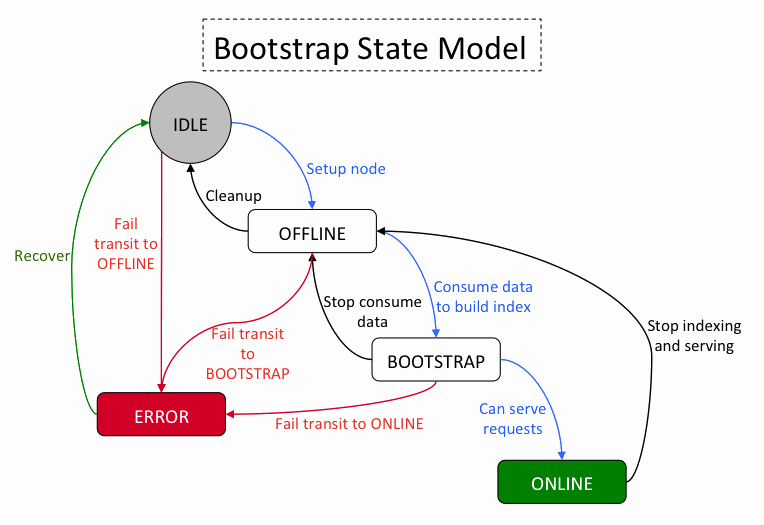
\includegraphics[width=\columnwidth]{bootstrap_statemodel.png}}
    \vspace*{-2ex}
    \caption{\label{fig:bootstrap_statemodel} \seas state machine.}
\end{figure}

Figure~\ref{fig:bootstrap_statemodel} shows the detailed state machine for \seas, another
\helix-managed DDS. As with \\ \ES, the state model and
constraints are configured in \helix. \seas has large number
number of replicas and one of the main optimization goal is to throttle the
maximum number of \\
offline$\rightarrow$bootstrap transitions. 

\subsection{\helix Execution}
%
Thus far we have described how DDSs declare their behavior within \helix.  We
now describe how \helix invokes that behavior on behalf of the DDS at run-time.  
\helix execution is a matter of continually monitoring DDS state and, as
necessary, ordering transitions on the DDS.   There are a variety of changes 
that can occur within a system, both planned and unplanned: bootstrapping the
DDS, adding or losing nodes, adding or deleting resources, adding or deleting
partitions, among others (we discuss detecting the unplanned changes in
Section~\ref{sec:arch}).

\begin{algorithm}
\label{alg:execution}
\caption{\helix execution algorithm}
\begin{algorithmic}[1]
\REPEAT
\STATE validTrans = $\emptyset$
\STATE inflightTrans = $\emptyset$
\FOR {each partition $p_i$}
  \STATE Read currentState
  \STATE Compute targetState 
  \STATE Read $p_i$ pendingTrans
  \STATE inflightTrans.addAll(pendingTrans)
  \STATE requiredTrans = computeTrans(currentState, targetState, 
pendingTrans) 
  \STATE validTrans.addAll(getValidTransSet( \\ requiredTrans))
\ENDFOR
\STATE newTrans = throttleTrans(inflightTrans, validTrans) 
\UNTIL {newTrans == $\emptyset$}
\end{algorithmic}
\end{algorithm}

\eat{%%%%%%%%%
\begin{algorithm}
\label{alg:changeset}
\caption{getPrioritizedValidTransitionSet algorithm.}
\begin{algorithmic}
\STATE pending = $\emptyset$
\STATE Sort requiredTransitions descending by priority
\STATE \FOR {each transition $t_i$ in sorted list}
\STATE \IF (! isViolated(pending, $t_i$)) 
\STATE 	pending.add($t_i$)
\STATE \ENDIF
\STATE \ENDFOR
\end{algorithmic}
\end{algorithm}

\begin{algorithm}
\label{alg:throttle}
\caption{Throttled transition execution.}
\begin{algorithmic}
\STATE FILL THIS IN
\end{algorithmic}
\end{algorithm}
}%%%%%%%%%%%%%

\eat{%%%%%%%%
\begin{algorithm}
\caption{\helix execution algorithm, run anytime a cluster becomes invalid.}
\begin{algorithmic}
\STATE //Compute all transitions
\FORALL {partitions $p_i$}
	 \STATE initialize transition set $T(p_i)=\{\}$
         TODO: write how we compute transitions
\ENDFOR
\STATE //Create per-partition batches
\STATE //Parallel execute batches with optional throttling
\end{algorithmic}
\end{algorithm}
}%%%%%%%%

The most crucial feature of the \helix transition algorithm is that it is identical 
across all of these changes and across all DDSs!  Else, we face a great deal of
complexity trying to manage so many combinations of changes and DDSs, and lose
much of \helix's generality.   
The execution algorithm appears in Algorithm~\ref{alg:execution} and we now step
through it.


In lines 2-3 we initialize two transition sets: validTrans and
inflightTrans, whose purposes we describe shortly.  
The first step, in lines 5-6, is on a partition-by-partition basis, to 
read the DDS's current state and compute a target state, where
target state is a distribution of a partition's replicas over cluster nodes 
that respects the DDS's constraints and optimization goals.  Most of the time, 
the current state will match the target state, and there is nothing to do; they
disagree only when the cluster changes (e.g. nodes lost, partitions added,
\etc).

By default we use the RUSH~\cite{honicky04} algorithm to produce the target state,
though with enhancements to ensure we meet state machine constraints and to
ensure we meet our optimization goals.  Default RUSH relies on
random hashing of a huge number of partitions to meet load balancing goals.
Since DDSs can have as few as 10s of partitions per node, to avoid load skew and
so better meet optimization goals, we
additionally assign each node a budget that limits the number of partitions it
may host.  \helix makes it easy to plug in other algorithms; we
discuss this more in Section~\ref{sec:placement}.

Given a partition's target state, line 7-9 reads all pending transitions for the
partition and then computes necessary additional replica transitions.
Given current state and the state model, producing the set of all necessary
transitions is straightforward
and we omit the details.

The next part of the algorithm computes a set of valid transitions for the
partition, taking into account the already pending transitions and those that
still must occur.  Our key insight is that when we trigger multiple transitions
in parallel, these transitions are not instantaneous and we do not know in what
order they will complete.  if we simply trigger any arbitrary
set of transitions (including all of them), it could violate system
constraint(\eg having more than one master) while they are underway.  In
contrast, if we issue transitions one-at-a-time, we know the exact states of the partition, but then progress through the transitions very slowly.

Our solution is to produce valid \emph{transition sets}; for a given
partition, a transition set is valid if
for every possible ordering of its transitions, the partition remains valid.    
Line 10 calls a method getValidTransSet that initializes a
transition set to include all
currently pending transitions for a partition and greedily adds other required
transitions, as long as the transition set remains valid, until no more
transitions can be added.  It considers the transitions in priority order,
according to the optimization goals given by the DDS.

Note we compute transition sets partition-by-partition.  Since the AFSM is
per-partition, we can safely execute a valid transition set per each partition
without making any partition invalid.  Thus, we have two potential dimensions for
parallelism: by building transition sets per partition, and across partitions.

By line 12 we have a set of valid transitions to run
across all partitions.  We do not simply execute them all, but instead now take
into account the DDS's throttling optimization goals.  The throttleTransitions
method takes the set of all inflight transitions (from prior rounds) and then
selects as many additional transitions as possible, without violating
constraints.  Notice that any non-scheduled valid transitions are essentially
forgotten and are considered anew in later rounds.

Finally, not shown in the algorithm is what happens when transitions complete.
We are notified by callback and remove those transitions from their partitions
lists of pending transitions.

The execution algorithm has two greedy key steps, to produce valid transitions and to
choose transitions for execution, rather than deriving both in a single
optimization.
While we could combine the two to produce a provably optimal solution, for the
time being, we find the current approach produces a high level of parallelism,
with highest priority transitions scheduled early.

\subsubsection{Application-Customized Execution}
\label{sec:placement}
%
By default \helix places replicas using modified RUSH, as described in
Algorithm~\ref{alg:execution}.  We refer to this as \emph{auto} placement.  
While this approach makes things very simple for some applications, it may not
be powerful enough for all applications, such as those that want to customize
placement of a single resource's partitions or even control placement of
multiple resources' partitions. 
\helix offers a pluggable interface 
that lets DDSs customize placement.  \emph{Semi-auto} placement lets DDSs decide
replica placement, while \helix still chooses the states of those replicas.
\emph{Custom} placement lets DDSs fully customize placement and state.

There are a number of reasons an application may want more explicit control over
\helix's decisions.  They might have application-specific requirements that
cannot currently be expressed in \helix.  For example, HBase can use \emph{semi-auto}
placement to co-locate its regions servers with the HDFS blocks
containing those regions' data.  

Finally, applications may also simply want explicit
control over all placement, because they are very specialized, or because they
are wary of handing over all control to \helix.   We do not want to turn away
such applications, and so permit customized placement in \helix, while allowing
them to benefit from all of \helix's other features, rather than 
force such applications to build their own cluster management from scratch.


%\begin{figure*}[t]
%{\includegraphics[width=0.9\textwidth]{figs/execution_example.png}}
%\caption{Example of \helix execution algorithm.}
%\end{figure*}

\subsubsection{Execution example}
%
We consider a case when a node is added to already existing
cluster to illustrate the execution sequence in Helix.
Suppose we start with an \ES cluster with 3 nodes $n_0 \ldots n_2$, 12
partitions $p_0 \ldots p_{12}$, and a replication level of 3; there are 12 total
replicas per node.  We then add a node $n_3$. 
Intuitively, we want to rebalance the cluster such that every node is left with
9 replicas.  In \helix execution we first compute a target state for each
$p_i$.  For 9 of 12 partitions the target state differs from the current state.  In
particular, 3 partitions get mastered on the new node and 6 partitions get
slaved on the new node.  We compute the required transitions for each partition.
Suppose $p_{10}$ will have its master replica moved from $n_1$ to $n_3$.  $n_1$
must execute $t1=(M \rightarrow S$) for $p_{10}$, while $n_3$ must execute $t2=(O
\rightarrow S)$ and $t3=(S \rightarrow M)$.  We cannot, however, execute these
transitions all in parallel since some orderings make the system invalid.
In order to avoid $p_{10}$ being mastered twice, $t3$ must execute only after
$t1$ completes. Helix automatically enforces this since it
issues a transition if and only if it does not violate any of the
state constraints. There are two possibile valid groupings to reach this target
state. One is to execute $t1$ and $t2$ in
parallel, and then execute $t3$, while the other is to execute $t2$, $t1$, and $t3$
sequentially. Helix chooses
the first approach.
 
Across all partitions, we produce
a set of 18 valid transitions that we can execute in parallel; however, since 
this \ES cluster prohibits more than 10 from running in parallel, 
we produce a transition set of size 10, and save all remaining transitions
(delayed due to validity or throttling) to later rounds. Its important to note that
Helix does not wait for all 10 transitions to complete before issuing the
remaining transitions. Instead, as soon as the first transition is completed, it
reruns the execution algorithm and tries to issue additional transitions. 

\eat{%%%%%%%
that makes transition decisions is identical across all
DDSs.  Faced with all these changes, \helix uses the DDS-provided AFSM to
first check whether the DDS is in a valid configuration and second, if not, initiate transitions to
make it valid.  These two steps constitute a tight feedback look that \helix
executes until the DDS is valid.

Since partitions are the DDS's lowest level of state granularity and are
mutually independent, \helix runs the execution algorithm against each partition
separately.  The execution algorithm is as follows:
}%%%%%%%%%




\eat{%%%%%%%%
\helix supports constraints at multiple granularities. 
Partition
Resource
Node
Cluster
These constraints can be applicable either to a STATE or a TRANSITION.
This feature of being able to specify constraint at various granularities is
proven to be quite useful to achieve important requirements such as
partition placement, throttling, load balancing etc. 
}%%%%%%%%%%%%%

\eat{%%%%%%%
Before we describe how these constraints can be used to
solve system specific requirements, lets recap the two important things need to
happen in \helix given an AFSM
1) Compute the Partition,State to Node mapping such that constraints will be satisfied. 
2) Once the mapping is computed, issue transitions to the nodes such that constraints are not violated.
Now lets see how Helix achieves these two functionalities
\subsubsection{Partition Mapping Module}
\label{sec:partitionmappingmodule}
Apart from satisfying simple constraints on the state machine such as
Number of Master=1, Number of Slaves=3 there can be more constraints that this
assignment needs to satisfy.
For example, as we see in Espresso use case, the assignment has to satisfy the 1) Master partitions are
evenly distributed among the nodes 2) (1) has to hold good even after nodes
fail/add.
}%%%%%%%%%%%%

\eat{%%%%%%%%
Helix automatically comes with few generic assignment algorithms that solves
most of the assignment problems. It supports multiple modes
1) Auto: In this mode the (partition,state) -> (Node) assignment is automatically
calculated for every change in the cluster state. Lets
consider the requirements of Espresso to distribute Master Partitions
equally among the nodes in the cluster. This constraint can be provided to
Helix as max number of master partitions per node=Total number of
partitions/Alive Nodes. This constraint ensures that the
(partition,state)->(node) solution computed by Helix solves requirement 1) and
2).
Another interesting but quite useful that automatically comes with Helix is it tries to minimize the transitions required in the system to reach the stable state. 
There are two interesting cases to that will make explain this in detail. When a
master fails there are two solutions possible. 
Node Failure:
One is to promote a partition
which is currently in Slave state for that partition. The other solution is to
assign this partition to a new node. Helix automatically chooses the first
solution since it requires the minimum transition. This is achieved by
specifying the following constraints.
a Max partition per node = Total partition*Number of Replicas/Nodes. 
b) Number of Slaves is between 0 and 3.
The denominator of this constraint a) is very important, what this means is once
the partition->Nodes mapping is computed it never changes until new nodes are added
to the system. This is very important to stateful data
systems like Espresso where creation/removal of a partition is expensive. Constraint b) is provided so that Helix knows that system can
be stable with less number of slaves. Lets say that Espresso has to change
this behavior in future such that new replicas are automatically created all it
needs to do is change is 
a) Max partition per node=(Total partition*Number of Replicas)/Alive Nodes. 
b) Number of Slaves is 3.

Node addition
New nodes are added to system to handle more load, this is simple way to
scale the system since some partitions now can be hosted on the new nodes. One
problem is here what partitions should be moved to the new nodes. This operation
generally known as rebalancing is often not thought of carefully in most DDS.
This operation ends up being very expensive, manual and laborious. Helix provides
three important features here, automation, throttling and minimizing partition
shuffling and downtime. Automation comes
naturally because of the state machine approach. The algorithm that computes the
assignment of partition,state-> node automatically tries to minimize the number of
transitions required to system from current state to new state.  Downtime can be
minimized by prioritizing transitions. In case of Espresso, when new node(N2) is
added and it is supposed to become Master for Partition P1 which is currently
mastered at N1. The followings transitions need to happen on P1.
t1 N1 -> M-S 
t2 N2 ->O-S
t3 N2-> S-M

There are two ways these transitions can be fired in multiple groups. 
t1, t2 and then t3
t2 and then t1 and then t3

If all transitions take equal amount of time then first solution is faster since
t1 and t2 can happen in parallel and t3 can be fired as soon as t1 and t2 is
completed. Though this solution looks attractive, it will result in larger
downtime since O-S generally takes more time since it has to do bootstrap of P1
which might involve copying large data. This can be easily achieved in Helix by
prioritizing the transitions. For example, prioritizing transitions in order of
S-M, O-S, M-S will ensure that downtime is minimum. <K>(Need to verify this)<K>

Another important thins needed in distributed system but often ignored until a
catastrophe is throttling. For example, when new nodes are added there will be
massive amount of bootstrapping that will move data around in the system. This
process if not controlled can bring down the entire cluster.
One can simply make use of this feature by saying
Max offline to slave transition per node=3.
max offline to slave transition in cluster=10
It is important to have the ability to specify the constraints at multiple
granualarities based on the system capacity.

 
 
3) Custom: We have seen that most cases the Auto mode is sufficient, but
in some cases system might have their own custom logic to decide the
(partition,state)->(node) assignment. In these cases, Helix supports Custom mode
where the application can plugin their custom code to dictate the
assignment.Custom mode simply means that Assignment is provided externally,
Helix still does the heavy lifting of issuing the transitions and ensuring
constraints on State are not violated and transition constraints are satisfied.
\aes{This section is missing, need to fill this in.}
\aes{This section must talk about how this works when we have load-imbalance due
to skew or whatever.  If you knew weights of partitions have changed, what do
you do?  \helix must observe this (through monitoring) and then act.}
}%%%%%%%%%%%%%


